    %---------------------------------------------------------------
        %% MLP-Algorithm
        %-----------------------------------------
\begin{tikzpicture}[>=stealth', node distance=\layersep cm, shorten >=1pt]
        \def\layersep{1.8}            % vertikal distance between the layers
        \def\neuronsep{1.8}         % Horizontal distance between neurons
        \def\dlsize{2}            % distance between node and layer lable
        \def\inout{\layersep*.65}   % Size of in- and output-arrow
        \def\siz{.8}                % neuronsize
        \def\y{5}                   % Start of the most upper layer
        \def\ni{2}                  % Amount of input neurons
        \def\nh{3}                  % Amount of hidden neurons
        \def\no{2}                  % Amount of output neurons
        \tikzstyle{neuron}=[circle,draw=black,minimum size=\siz cm,inner sep=2pt]
        \tikzstyle{annot} = [text width=6em, text centered]
        \tikzset{fontscale/.style = {font={\fontsize{#1pt}{#1pt}\selectfont}}}

        \newcommand{\neurono}[2][]{
            \node[neuron,circle split,inner sep=2pt] (#1) at (#2)
                    {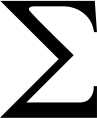
\includegraphics[width=0.225cm]{Bilder/Sigma.png} \nodepart{lower} 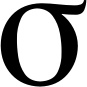
\includegraphics[width=0.225cm]{Bilder/sigma.png}};
        }
        % Draw the left input layer nodes
            \foreach \name / \xn in {1,...,\ni}{
            % This is the same as writing \foreach \name / \y in {1/1,2/2,3/3,4/4}
                \node[neuron,fontscale=15] (Il-\name) at (\xn*\neuronsep-\neuronsep,\y) {$X_{\xn}$};
                \node[above of=Il-\name, node distance=\inout cm] (Inl-\name) {};
                \draw [->,arrows={-Stealth[length=7pt]},densely dotted] (Inl-\name) edge (Il-\name);
            }
            \node[fontscale=15] (Il-dot) at ({(\ni+1)*\neuronsep-\neuronsep},\y) {$\dots$};
            \node[neuron,fontscale=15] (Il-i) at ({(\ni+2)*\neuronsep-\neuronsep},\y) {$X_{i}$};
            \node[above of=Il-i, node distance=\inout cm] (Inl-i) {};
            \draw [->,arrows={-Stealth[length=7pt]},densely dotted] (Inl-i) edge (Il-i);

        % Draw the hidden layer node
            \foreach \name / \xn in {1,...,\nh}{
                \node[neuron] (Hl-\xn) at ({(\ni-1)*\neuronsep/2-\neuronsep/2*(\nh-1)+(\xn-1)*\neuronsep},\y-\layersep) [fontscale=15] {$Z_{\xn}$};
                
                \node[node distance=\inout cm, below of=Hl-\xn] (Hnl) {};
                %\draw [->,arrows={-Stealth[length=7pt]},densely dotted] (Hl-\xn) edge (Hnl);
            }
                \node[fontscale=15] (Hl-dot) at ({(\ni-1)*\neuronsep/2-\neuronsep/2*(\nh+1)+(\nh+1)*\neuronsep},\y-\layersep) {$\dots$};
                \node[neuron,fontscale=15] (Hl-h) at ({(\ni-1)*\neuronsep/2-\neuronsep/2*(\nh+2)+(\nh+2.5)*\neuronsep},\y-\layersep) {$Z_h$};
            
            \foreach \name / \xn in {1,...,\nh,h}{
        % Connect every node in the inner layer with the hidden layer
            \foreach \source in {1,...,\ni,i}
                \draw [->,arrows={-Stealth[length=7pt]}] (Il-\source) edge (Hl-\xn);
                }
                \draw [fill=white,draw=black, dotted] ($(Hl-1)+(\neuronsep/4-.45,\layersep*.625)$) rectangle ($(Hl-h)+(\neuronsep/100,\layersep*.4)$);
                \node[fill=white,inner sep=1pt,fontscale=10] at ($(Hl-1)+({(\nh+1)*\neuronsep/2},\layersep*.5)$) {$\dots\,w_{h,i}\,\dots$};

        % Draw the output layer node
            \foreach \name / \xn in {1,...,\no}{
                \node[neuron,fontscale=15] (Ol-\xn) at ({(\ni-1)*\neuronsep/2-\neuronsep/2*(\no-1)+(\xn-1)*\neuronsep},\y-2*\layersep) {$Y_{\xn}$};
                \node[node distance=\inout cm, below of=Ol-\xn] (Onl) {};
                \draw [->,arrows={-Stealth[length=7pt]},densely dotted] (Ol-\xn) edge (Onl);
            }
                \node[fontscale=15] (Ol-dot) at ({(\ni-1)*\neuronsep/2-\neuronsep/2*(\no+1)+(\no+1)*\neuronsep},\y-2*\layersep)  {$\dots$};
                \node[neuron,fontscale=15] (Ol-o) at ({(\ni-1)*\neuronsep/2-\neuronsep/2*(\no+2)+(\no+2.5)*\neuronsep},\y-2*\layersep)  {$Y_o$};
                \node[node distance=\inout cm, below of=Ol-o] (Onl) {};
                \draw [->,arrows={-Stealth[length=7pt]},densely dotted] (Ol-o) edge (Onl);
            
            \foreach \name / \xn in {1,...,\no,o}{
        % Connect every node in the hidden layer with the output layer
            \foreach \source in {1,...,\nh,h}
                \draw [->,arrows={-Stealth[length=7pt]}] (Hl-\source) edge (Ol-\xn);
                }
                \draw [fill=white,draw=black, dotted] ($(Ol-1)+(\neuronsep/3-1.5,\layersep*.625)$) rectangle ($(Ol-o)+(\neuronsep/2,\layersep*.4)$);
                \node[fill=white,inner sep=1pt,fontscale=10] at ($(Ol-1)+({(\no+1)*\neuronsep/2},\layersep*.5)$) {$\dots\,w_{o,h}\,\dots$};
                
        % Annotate the layers
            \ifthenelse{\ni>\nh}{
                \node[annot,right of=Il-i, node distance=\dlsize cm] (il) {\textbf{Eingabe- schicht}};
                \node[annot,below of=il] (hl) {\textbf{Verdeckte- schicht}};
            }{
                \node[annot,right of=Hl-h, node distance=\dlsize cm] (hl) {\textbf{Verdeckte- schicht}};
                \node[annot,above of=hl] (il) {\textbf{Eingabe- schicht}};
            }
                \node[annot,below of=hl] {\textbf{Ausgabe- schicht}};            
\end{tikzpicture}